\documentclass{article}
\usepackage[margin=.6in]{geometry}
\usepackage{amsmath,amsfonts,amssymb,mathtools}
\usepackage{enumerate}
\usepackage{physics}
\usepackage{graphics,graphicx,epstopdf}
\usepackage[dvipsnames]{xcolor}
\usepackage{float}
\setlength\parindent{0pt}

\newcommand{\R}{\mathbb{R}}
\newcommand{\N}{\mathbb{N}}
\newcommand{\Z}{\mathbb{Z}}
\newcommand{\T}{\mathbb{T}}
\newcommand{\Q}{\mathbb{Q}}
\newcommand{\D}{\mathbb{D}}
\newcommand{\e}{\mathrm{e}}
\newcommand{\C}{\mathbb{C}}

\newcommand{\figlabel}[1]{\textbf{(#1)}}

\newcommand{\comment}[1]{\textsc{\color[rgb]{1,0,0}#1}}

\title{Principal Component Analysis for Semantic Classification \\ AMATH 582 Final Project}
\author{Benjamin Liu, Kelsey Maass, and Riley Molloy}
\begin{document}

% Title/author/abstract
\maketitle
\bigskip

% Abstract
\abstract{Principal component analysis (PCA) and classification by supervised learning are two popular topics in data science today. In this article, we combine techniques from both areas in order to classify news articles based on their word frequency content. We find that we can accurately classify the data by projecting onto a small subset of principal components, reducing the feature space from nearly $10 \,000$ elements to just four. We also compare results from the traditional and robust PCA formulations, and discuss what additional semantic information can be inferred from our results.}


% Sec 1. Introduction and Overview
\section{Introduction and Overview}
PCA and Robust PCA


% Sec 2. Theoretical Background
\section{Theoretical Background}

\subsection{Principal Component Analysis}
\begin{align}
A &= U S V^*
\label{eq:svd}
\end{align}

\subsection{Robust PCA}
\begin{align}
\min_{L,S} \norm{A-L-S}_{F}^2 + \lambda_1 \norm{L}_* + \lambda_2 \norm{S}_1,
\label{eq:robust_obj}
\end{align}
where $\norm{\cdot}_*$ is the nuclear norm, defined by
\begin{align*}
\norm{\cdot}_* = \norm{\sigma(\cdot)}_1
\end{align*}
where $\sigma$ maps a matrix to a vector of its singular values. Therefore the nuclear norm of a matrix is the sum of its singular values. In addition, $\norm{\cdot}_1$ is the vectorized $\ell_1$ norm, treating $S \in \R^{m \times n}$ as a vector in $S \in \R^{mn}.$

\subsection{Classification Methods}
% Sec 3. Algorithm Implementation and Development
\section{Algorithm Implementation and Development}

\subsection{Article Data}

\comment{Algorithm for turning articles into wordcount / wordfrequency data. Stemming, low wordcount removal, stopwords.}

\subsection{Robust PCA}

\subsection{Classification Schemes}

\subsubsection{Nearest Mean}

\subsubsection{K-Nearest Neighbors (KNN)}

\subsubsection{Logistic Regression}

\subsubsection{Neural Network}

\subsubsection{Support Vector Machine}

% Sec 4. Computational Results
\section{Computational Results}

\subsection{PCA and Robust PCA}
\begin{figure}[H]
\centering
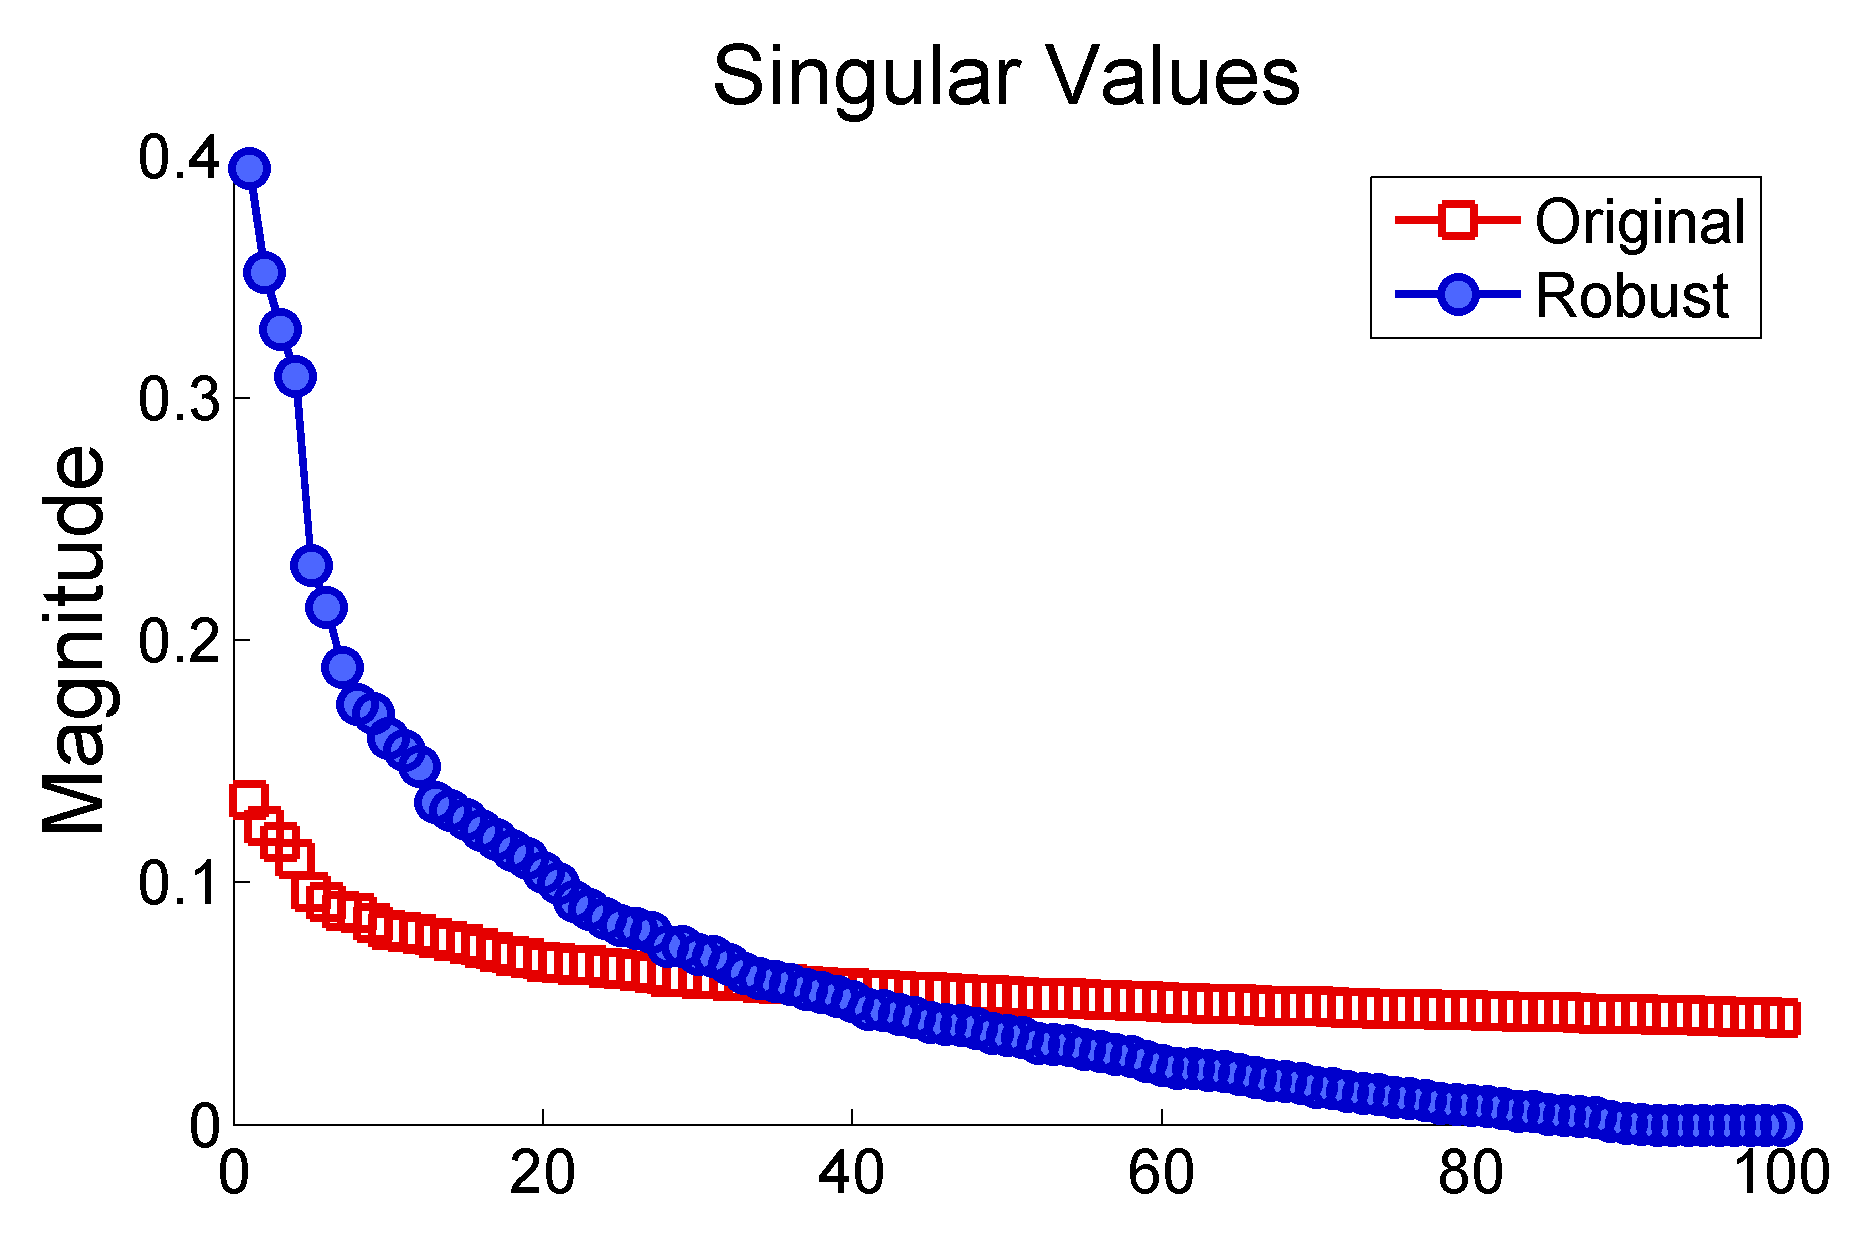
\includegraphics[width=.6\textwidth]{singularvaluescompare}
\end{figure}

\subsection{Classification}

% Sec 5. Summary and Conclusions
\section{Summary and Conclusions}

\newpage
% App A. MATLAB functions used and brief implementation explanation
\section*{Appendix A: MATLAB Functions}

\paragraph{ind = knnsearch(Xtrain,Xtest,k)} Finds the \textbf{k} elements of \textbf{Xtrain} that are nearest to \textbf{Xtest}, and returns the indices of these elements in \textbf{ind}.

\paragraph{svmtrain}

\paragraph{svmdecision}

% App B. MATLAB codes
\section*{Appendix B: MATLAB Codes}

% App C. (optional) Any algebraically intense calculations (long and drawn out calculations that have no business in Sec 2)
% \section{Appendix C}

\end{document} 